\chapter{Ising-Korrelationen, mittleres Feld und spontane Magnetisierung}

\lectureoverview{Eine eindimensionale Ising-Kette lässt sich exakt lösen, indem man die Spins an den Gitterplätzen durch Bindungsvariablen ersetzt. Diese Variablentransformation macht die Zustandssumme zu einem Produkt und zeigt, dass jede Korrelation bei endlicher Temperatur exponentiell abklingt. Höherdimensionale Gitter verhalten sich anders, weil jeder Spin Informationen von vielen Nachbarn erhält. Behandelt man ihren Gesamteinfluss als mittleres Feld, erhält man eine Selbstkonsistenzgleichung, eine kritische Temperatur im mittleren Feld und eine präzise Beschreibung dafür, wie ein beliebig kleines äußeres Feld eine der magnetisierten Phasen auswählt.}

\section{Was Ising tatsächlich herausfand}

Der historische Sachverhalt sollte korrekt dargestellt werden. Ernst Ising löste das eindimensionale Modell, das Wilhelm Lenz ihm vorgegeben hatte, und fand zutreffend keinen Phasenübergang bei endlicher Temperatur. Zu weit ging er mit der Schlussfolgerung, dass dasselbe Ergebnis in jeder Dimension gelten müsse. Das ist nicht der Fall. Bereits das zweidimensionale Modell besitzt eine geordnete Phase bei niedrigen Temperaturen.

Eine exakte Lösung in höherer Dimension wäre für den vorliegenden Zweck zu anspruchsvoll. Eine physikalisch anschauliche Näherung genügt, um den Übergang sichtbar zu machen, wenn jeder Spin viele Nachbarn hat. Bevor wir diese Näherung verwenden, lohnt es sich jedoch, die eindimensionale Kette exakt zu lösen. Der Vergleich zwischen der exakten eindimensionalen Antwort und der Näherung für hohe Dimensionen zeigt, welcher Mechanismus in einer Dimension fehlt.

Ein Phasenübergang bedeutet hier mehr als eine allmähliche Verstärkung einer bereits bestehenden Bevorzugung. Überschreitet die Temperatur einen kritischen Wert, erhält der Gleichgewichtszustand eine neue makroskopische Eigenschaft: Eine von null verschiedene Magnetisierung kann bestehen bleiben, selbst nachdem das äußere Feld entfernt wurde, mit dem die Probe ausgerichtet wurde. Die Rechnung muss daher zwei getrennte Fragen beantworten. Bewahrt ein weit entfernter Spin die Orientierung eines ausgewählten Spins, und kann ein infinitesimales Feld eine beliebig große Probe ordnen?

\section{Ein Spin als wiederverwendbarer Grundbaustein}

Betrachten wir eine Variable mit zwei Zuständen
\begin{equation}
\sigma=\pm1,
\end{equation}und wählen die Energiekonvention
\begin{equation}
E(\sigma)=-J\sigma,
\qquad J>0.
\end{equation}
Der Zustand \(\sigma=+1\) hat dann die niedrigere Energie. Der Parameter \(J\) kann für das Produkt aus magnetischem Moment und angelegtem Feld stehen; in diese Rechnung geht jedoch nur das Produkt ein.

Wir betrachten diesen Spin als kleines Teilsystem im thermischen Gleichgewicht mit allem Übrigen. Seine Zustandssumme lautet
\begin{align}
z
&=\sum_{\sigma=\pm1}e^{-\beta E(\sigma)}
 =\sum_{\sigma=\pm1}e^{\beta J\sigma} \\
&=e^{\beta J}+e^{-\beta J}
 =2\cosh(\beta J).
\end{align}

Dasselbe Ergebnis ließe sich auf eine Gesamtheit von \(N\) unabhängigen Spins übertragen. Die vollständige Zustandssumme wäre einfach \(Z=z^N\), also wäre \(\log Z=N\log z\) und jede extensive thermodynamische Größe das \(N\)-Fache ihres Werts für einen einzelnen Spin. Diese Betrachtung als Teilsystem ersetzt die längere kombinatorische Zählung der Spins, die nach oben oder unten zeigen, enthält aber dieselbe Information.
Die mittlere Energie ergibt sich aus der logarithmischen Ableitung:
\begin{align}
\expect{E}
&=-\frac{\partial}{\partial\beta}\log z \\
&=-J\frac{\sinh(\beta J)}{\cosh(\beta J)}
 =-J\tanh(\beta J).
\end{align}
Da \(E=-J\sigma\) gilt,
\begin{equation}
\expect{\sigma}=\tanh(\beta J).
\end{equation}

\begin{figure}[ht]
\centering
\includegraphics[width=0.80\textwidth]{lecture_09_figure_02.png}
\caption{Energie und Magnetisierung eines einzelnen Spins in der Form des hyperbolischen Tangens.}
\lectureframe{00:10:06}
\end{figure}

Diese eine Formel umfasst beide Temperaturgrenzfälle. Bei niedriger Temperatur gilt \(\beta J\gg1\), und der Spin befindet sich mit sehr hoher Wahrscheinlichkeit im Zustand niedrigerer Energie. Bei hoher Temperatur gilt \(\beta J\ll1\), sodass
\begin{equation}
\expect{\sigma}\simeq \beta J\longrightarrow0.
\end{equation}
Die thermische Bewegung hebt die energetische Bevorzugung auf.

\begin{classroomqa}
\audiencequestion{Müsste die mittlere Energie nicht ein Minuszeichen haben?}
\lecturerresponse{Ja. Die thermodynamische Identität lautet \(\expect{E}=-\partial_\beta\log z\), also ergibt sich \(-J\tanh(\beta J)\). Teilt man anschließend durch den Faktor \(-J\) in \(E=-J\sigma\), erhält man die positive Magnetisierung \(\expect{\sigma}=\tanh(\beta J)\). \lecturetimestamp{00:09:15--00:09:44}}
\end{classroomqa}

\section{Die eindimensionale Kette}

Wir ordnen \(N\) Spins auf einer offenen Kette an und lassen benachbarte Spins miteinander wechselwirken:
\begin{equation}
H=-J\sum_{i=1}^{N-1}\sigma_i\sigma_{i+1},
\qquad \sigma_i=\pm1.
\label{eq:ising-chain}
\end{equation}
Für \(J>0\) trägt ein paralleles Paar \(-J\) bei, ein antiparalleles Paar dagegen \(+J\). Die beiden Grundzustände sind daher
\begin{equation}
(+,+,\ldots,+)
\qquad\text{and}\qquad
(-,-,\ldots,-).
\end{equation}

\begin{figure}[ht]
\centering
\includegraphics[width=0.80\textwidth]{lecture_09_figure_03.png}
\caption{Der Hamiltonoperator der offenen Kette und die zugehörige Boltzmann-Summe.}
\lectureframe{00:19:15}
\end{figure}

Der Wechsel von \(J\) zu \(-J\) begünstigt alternierende Spins. Bei einer offenen Kette oder einer geraden periodischen Kette führt die Umdefinition
\begin{equation}
\widetilde{\sigma}_i=(-1)^i\sigma_i
\end{equation}
das Vorzeichen der antiferromagnetischen Kopplung auf das ferromagnetische zurück. Der Unterschied ist physikalisch, doch die Algebra der Zustandssumme ist in einer Dimension dieselbe. Die bekannte Ausnahme ist eine ungerade periodische Kette, da sie wegen der Frustration nicht alternieren kann.

\begin{classroomqa}
\audiencequestion{Gibt es im Hamiltonoperator der Kette ein äußeres Magnetfeld?}
\lecturerresponse{Noch nicht. Gleichung~\eqref{eq:ising-chain} enthält nur eine Kopplung zwischen nächsten Nachbarn. Später fügen wir ein homogenes äußeres Feld als separaten Term \(-h\sum_i\sigma_i\) hinzu, um gezielt zu prüfen, wie der geordnete Zustand auf eine beliebig kleine Bevorzugung reagiert. \lecturetimestamp{00:18:54--00:19:13}}
\end{classroomqa}

\subsection{Gedächtnis als Korrelationsfunktion}

Nehmen wir an, \(\sigma_i\) sei bekanntermaßen nach oben gerichtet. Beeinflusst diese Information einen Spin im Abstand von \(r\) Bindungen? Das Maß dafür ist
\begin{equation}
C(r)=\expect{\sigma_i\sigma_{i+r}}.
\end{equation}
Nähert sich \(C(r)\) für \(r\to\infty\) einem von null verschiedenen Wert, bewahrt das System eine langreichweitige Erinnerung. Nähert sich die Korrelation null, verschwindet der Einfluss des ersten Spins schließlich.

Das Stille-Post-Spiel liefert die passende Anschauung. Jede Person gibt ein binäres Symbol an die nächste weiter. Ist jede Übermittlung fehlerfrei, bleibt das ursprüngliche Bit unbegrenzt erhalten. Tritt bei jedem Schritt eine noch so kleine Fehlerwahrscheinlichkeit auf, geht die ursprüngliche Nachricht durch die wiederholte Übermittlung schließlich verloren. Die Temperatur null entspricht im Ising-Modell dem Fall fehlerfreier Übertragung. Bei jeder positiven Temperatur sind gelegentliche Abweichungen zwischen Nachbarn möglich.

Zur Veranschaulichung mit Zahlen nehmen wir an, dass eine einzelne Übertragung die Zuverlässigkeit \(0.99\) hat. Zwei fehlerfreie Übertragungen erfolgen mit Wahrscheinlichkeit \(0.99^2=0.9801\), und jeder weitere Schritt liefert einen zusätzlichen Faktor \(0.99\). Schon nach hundert Schritten treten häufig Fehler auf; nach zehntausend Schritten ist das Gedächtnis praktisch ausgelöscht. In der Ising-Kette verwendet man ein vorzeichenbehaftetes Maß der Zuverlässigkeit statt dieser Wahrscheinlichkeit für fehlerfreie Übertragung, doch die multiplikative Abnahme ist dieselbe Idee.

Die Analogie wird exakt, sobald man eine Wahrscheinlichkeit von einer Korrelation unterscheidet. Ist \(p\) die Wahrscheinlichkeit, dass benachbarte Spins übereinstimmen, gilt
\begin{equation}
\expect{\sigma_i\sigma_{i+1}}
=p-(1-p)=2p-1.
\end{equation}
Die Größe, die sich also von Bindung zu Bindung multipliziert, ist die überschüssige Zuverlässigkeit \(2p-1\), nicht \(p\) selbst.

\section{Bindungsvariablen und die exakte Zustandssumme}

Die entscheidende Variablentransformation beschreibt Beziehungen statt einzelner Spins:
\begin{equation}
\mu_i=\sigma_i\sigma_{i+1},
\qquad i=1,\ldots,N-1.
\label{eq:bond-variable}
\end{equation}
Jede Bindungsvariable ist bei übereinstimmenden Spins \(+1\) und bei unterschiedlichen Spins \(-1\). Ist der erste Spin festgelegt, bestimmen die Bindungen alle folgenden Spins:
\begin{align}
\sigma_2&=\sigma_1\mu_1,\\
\sigma_3&=\sigma_1\mu_1\mu_2,\\
\sigma_{r+1}&=\sigma_1\prod_{k=1}^{r}\mu_k.
\end{align}
Es gibt keine Redundanz. Die Daten \((\sigma_1,\mu_1,\ldots,\mu_{N-1})\) sind gleichwertig mit \((\sigma_1,\ldots,\sigma_N)\).

In diesen Variablen lautet die Energie einfach
\begin{equation}
H=-J\sum_{i=1}^{N-1}\mu_i.
\end{equation}
Aus den wechselwirkenden Variablen an den Gitterplätzen sind unabhängige Bindungsvariablen geworden. Summiert man zunächst über die beiden Werte von \(\sigma_1\), erhält man
\begin{align}
Z_N
&=2\sum_{\{\mu_i=\pm1\}}
\exp\left(\beta J\sum_{i=1}^{N-1}\mu_i\right)\\
&=2\prod_{i=1}^{N-1}
\left(\sum_{\mu_i=\pm1}e^{\beta J\mu_i}\right)\\
&=2\left[2\cosh(\beta J)\right]^{N-1}.
\label{eq:chain-partition}
\end{align}
Es gibt \(N-1\) Faktoren, denn eine offene Kette mit \(N\) Gitterplätzen hat \(N-1\) Bindungen.

Der führende Faktor zwei steht für die globale Wahl des ersten Spins. Er trägt nur \(\log2\) zu \(\log Z_N\) bei, während die Bindungen einen Term proportional zu \(N-1\) liefern. Für die exakte Zählung bei endlicher Größe ist der Faktor wichtig, doch für die freie Energiedichte verschwindet sein Beitrag im Grenzfall \(N\to\infty\). Deshalb konnte der Tafeltext ihn als „keine große Sache“ bezeichnen, ohne ihn tatsächlich wegzulassen.

\begin{figure}[ht]
\centering
\includegraphics[width=0.82\textwidth]{lecture_09_figure_04.png}
\caption{Der Hamiltonoperator in Gitterplatzvariablen, umgeschrieben als Summe über unabhängige Bindungen, und die daraus resultierende faktorisierte Zustandssumme.}
\lectureframe{00:35:35}
\end{figure}

\begin{classroomqa}
\audiencequestion{Was geschah mit der Summe im Exponenten, als die endgültige Antwort zu einer Potenz wurde?}
\lecturerresponse{Zunächst wurde daraus ein Produkt, und daraus wiederum eine Potenz:
\[
e^{\beta J\sum_i\mu_i}=\prod_i e^{\beta J\mu_i}.
\]
Die Summe über alle Bindungskonfigurationen zerfällt dann in eine Zweitermsumme für jede Bindung. Da jeder Faktor \(2\cosh(\beta J)\) ist, ergibt das Produkt die Potenz \((N-1)\). Schreibt man den Fall mit drei Spins und zwei Bindungen aus, wird die Faktorisierung ganz explizit. \lecturetimestamp{00:33:25--00:35:36}}
\end{classroomqa}

Dies ist eine einfache duale Beschreibung: Gekoppelte Variablen an den Gitterplätzen werden durch ungekoppelte Variablen auf den Bindungen ersetzt. Der Begriff \emph{Dualität} passt hier, weil dasselbe System zwei Beschreibungen mit sehr unterschiedlich wirkenden Freiheitsgraden besitzt. Bei einer offenen eindimensionalen Kette handelt es sich um eine exakte Variablentransformation.

In der Sprache des Gitters leben die ursprünglichen Variablen auf den Knoten und die neuen auf den Kanten. Die globale Wahl des ersten Spins ist die zusätzliche Angabe, die benötigt wird, um die Knoten aus den Kanten zu rekonstruieren. Dieser Austausch von Gitterplätzen und Bindungen ist ein einfaches Beispiel für ein Muster, das in der statistischen Mechanik höherer Dimensionen wesentlich mächtiger wird.

\subsection{Zuverlässigkeit zwischen nächsten Nachbarn}

Jede Bindung hat dieselbe Verteilung,
\begin{equation}
\begin{aligned}
\Pr(\mu=+1)&=\frac{e^{\beta J}}{2\cosh(\beta J)},\\
\Pr(\mu=-1)&=\frac{e^{-\beta J}}{2\cosh(\beta J)}.
\end{aligned}
\end{equation}
Folglich gilt
\begin{equation}
\expect{\mu_i}
=\expect{\sigma_i\sigma_{i+1}}
=\tanh(\beta J).
\label{eq:nearest-correlation}
\end{equation}

\begin{figure}[ht]
\centering
\includegraphics[width=0.80\textwidth]{lecture_09_figure_05.png}
\caption{Die Korrelation zwischen nächsten Nachbarn, ausgedrückt als Mittelwert der Bindungsvariablen.}
\lectureframe{00:36:52}
\end{figure}

Die Wahrscheinlichkeit, dass Nachbarn übereinstimmen, beträgt somit
\begin{equation}
p_{\rm same}
=\frac{1+\tanh(\beta J)}{2}.
\end{equation}
Bei positivem \(J\) ist sie größer als ein Halb; bei Temperatur null nähert sie sich eins, und bei unendlicher Temperatur beträgt sie ein Halb.

\begin{classroomqa}
\audiencequestion{Warum bedeutet eine positive Korrelation zwischen nächsten Nachbarn, dass die Spins parallele statt antiparallele Ausrichtung bevorzugen?}
\lecturerresponse{Für \(J>0\) hat eine parallele Bindung die Energie \(-J\), eine antiparallele dagegen \(+J\). Der positive Wert von \(\expect{\mu}\) besagt, dass \(\mu=+1\), also parallele Ausrichtung, häufiger auftritt. Ob die effektive Kopplung in einem realen Material ferro- oder antiferromagnetisch ist, hängt von seiner mikroskopischen elektronischen Struktur ab; die hier verwendete Vorzeichenkonvention beschreibt einen Ferromagneten. \lecturetimestamp{00:43:45--00:44:48}}
\end{classroomqa}

\begin{classroomqa}
\audiencequestion{Was geschieht mit dieser Korrelation bei sehr hoher Temperatur?}
\lecturerresponse{Für \(T\to\infty\) gilt \(\beta\to0\) und \(\tanh(\beta J)\to0\). Dann übermitteln selbst nächste Nachbarn keine Information mehr voneinander: Jeder Spin ist praktisch eine Zufallsvermutung. \lecturetimestamp{00:46:42--00:47:20}}
\end{classroomqa}

\subsection{Korrelation über große Abstände}

Für Spins, die durch \(r\) Bindungen getrennt sind, gilt
\begin{align}
\sigma_i\sigma_{i+r}
&=\sigma_i
\left(\prod_{k=i+1}^{i+r-1}\sigma_k^2\right)
\sigma_{i+r}\\
&=(\sigma_i\sigma_{i+1})
(\sigma_{i+1}\sigma_{i+2})\cdots
(\sigma_{i+r-1}\sigma_{i+r})\\
&=\prod_{k=i}^{i+r-1}\mu_k.
\end{align}
Da die \(\mu_k\) unabhängig sind,
\begin{equation}
C(r)=\expect{\sigma_i\sigma_{i+r}}
=\left[\tanh(\beta J)\right]^r.
\label{eq:exact-correlation}
\end{equation}

\begin{figure}[ht]
\centering
\includegraphics[width=0.80\textwidth]{lecture_09_figure_06.png}
\caption{Zwischenfaktoren \(\sigma_k^2=1\) verwandeln das Produkt der Spins an den entfernten Endpunkten in ein Produkt unabhängiger Bindungsvariablen.}
\lectureframe{00:41:35}
\end{figure}

\begin{classroomqa}
\audiencequestion{Die Korrelationsfunktion enthält nur die beiden Spins an den Endpunkten. Woher kommen all die Spins dazwischen?}
\lecturerresponse{Sie wurden lediglich als Faktoren gleich eins eingefügt: \(\sigma_k^2=1\). Durch paarweises Zusammenfassen benachbarter Faktoren wird das Produkt der Endpunkt-Spins in Bindungsvariablen umgeschrieben, deren thermische Verteilung genau faktorisiert. Der Wert der Korrelationsfunktion bleibt dabei unverändert. \lecturetimestamp{00:41:41--00:42:26}}
\end{classroomqa}

Bei jeder endlichen Temperatur gilt
\begin{equation}
0<\tanh(\beta J)<1,
\end{equation}
Das Gedächtnis klingt also exponentiell ab. Die Schreibweise
\begin{equation}
C(r)=e^{-r/\xi}
\end{equation}
definiert die exakte Korrelationslänge
\begin{equation}
\xi^{-1}=-\log\!\left[\tanh(\beta J)\right].
\label{eq:correlation-length}
\end{equation}
Nur bei \(T=0\) divergiert \(\xi\). Bei niedriger, aber von null verschiedener Temperatur gilt
\begin{equation}
\xi\simeq \frac{1}{2}e^{2\beta J},
\end{equation}
Die Kette kann daher sehr lange parallele Abschnitte enthalten, ohne eine echte Fernordnung zu besitzen.

Die Kette wirkt daher verklumpt. Man sieht eine lange Folge nach oben gerichteter Spins, dann einen Wechsel, dann eine lange Folge nach unten gerichteter Spins und anschließend einen weiteren Wechsel. Bei niedriger Temperatur sind diese Abschnitte lang, weil eine Domänenwand selten ist; ganz verschwinden Domänenwände dadurch aber nicht. Für Magnetisierung braucht man eine unendliche Gedächtnislänge, nicht bloß eine sehr große.

\section{Warum eine größere Zahl von Nachbarn das Problem verändert}

In einer Dimension gibt es keine Fehlerkorrektur. Sobald eine Bindung von ihrem Vorgänger abweicht, gibt es für den nächsten Spin keine unabhängige Information darüber, welche Orientierung beabsichtigt war. Die Kette besteht deshalb aus langen parallelen Domänen, die durch gelegentliche Wechsel getrennt sind.

Auf einem quadratischen Gitter hat jeder Gitterplatz vier nächste Nachbarn. Auf einem kubischen Gitter sind es sechs. Auf einem \(d\)-dimensionalen hyperkubischen Gitter hat er
\begin{equation}
z=2d
\end{equation}
nächste Nachbarn. Ein Gitterplatz, der drei übereinstimmende und eine abweichende Information erhält, kann der Mehrheit folgen. Die Umgebung mit vielen Nachbarn unterdrückt vereinzelte Fehler ähnlich wie redundante Nachrichten eine Fehlerkorrektur ermöglichen.

Haben die Nachbarn den mittleren Spin \(m\), so hat ihre Summe den Mittelwert \(zm\). Ihre gewöhnliche Fluktuation ist von der Größenordnung \(\sqrt{z}\), sodass die relative Fluktuation für Werte abseits von \(m=0\) näherungsweise wie folgt skaliert:
\begin{equation}
\frac{\sqrt{z}}{z|m|}
=\frac{1}{\sqrt{z}\,|m|}.
\end{equation}
Deshalb ist die Näherung durch ein mittleres Feld bei großer Koordinationszahl plausibel. Zugleich zeigt sich daran, dass sie nahe einem kritischen Punkt am wenigsten zuverlässig ist, denn dort ist \(m\) klein.

Ein bekanntes Sprichwort bringt die Intuition für große Zahlen auf den Punkt: Bei hundert unabhängigen Stimmen ist es unwahrscheinlich, dass sie alle in dieselbe falsche Richtung weisen. Die quantitative Fassung ist das Wurzelgesetz. Eine kohärente Verzerrung bei \(z\) Variablen ist proportional zu \(z\), während die zufällige Abweichung typischerweise nur proportional zu \(\sqrt{z}\) ist. Eine höhere Dimension verändert daher nicht nur die Zahl der Nachbarn, sondern auch die Zuverlässigkeit ihrer gemeinsamen Information.

\begin{classroomqa}
\audiencequestion{Entsprechen Dimensionen über drei hinaus einem physikalischen magnetischen Material?}
\lecturerresponse{Nicht unmittelbar als räumliche Dimensionen. Ein großes \(d\) ist ein lösbarer Grenzfall, in dem jeder Gitterplatz viele Nachbarn hat und die Mittelung kontrolliert wird. Ist der Mechanismus dort sichtbar, kann man fragen, wie weit er sich auf die physikalischen Dimensionen übertragen lässt. Beim Ising-Modell reichen bereits zwei Dimensionen für einen Phasenübergang bei endlicher Temperatur, auch wenn das mittlere Feld die zweidimensionale Antwort nicht exakt liefert. \lecturetimestamp{00:52:32--00:53:50}}
\end{classroomqa}

\section{Das mittlere Feld als Selbstkonsistenzproblem}

Betrachten wir einen Spin \(\sigma_i\). Seine Wechselwirkung mit den \(z=2d\) Nachbarn lautet
\begin{equation}
E_i=-J\sigma_i\sum_{j\in{\rm nn}(i)}\sigma_j.
\label{eq:local-energy}
\end{equation}
Sei
\begin{equation}
m=\expect{\sigma}
\end{equation}
die homogene Magnetisierung pro Spin. Im mittleren Feld wird die fluktuierende Summe über die Nachbarn durch ihren Mittelwert ersetzt:
\begin{equation}
\sum_{j\in{\rm nn}(i)}\sigma_j
\longrightarrow zm=2dm.
\end{equation}
Der ausgewählte Spin hat dann die effektive Energie eines einzelnen Spins
\begin{equation}
E_i^{\rm MF}=-2dJm\,\sigma_i.
\label{eq:mean-field-energy}
\end{equation}

\begin{figure}[ht]
\centering
\includegraphics[width=0.82\textwidth]{lecture_09_figure_07.png}
\caption{Ein ausgewählter Spin, seine \(2d\) nächsten Nachbarn und der Ersatz ihrer Summe durch die mittlere Magnetisierung.}
\lectureframe{01:00:30}
\end{figure}

Nun lässt sich das Ergebnis für einen einzelnen Spin mit dem effektiven Feld \(2dJm\) wiederverwenden:
\begin{equation}
\expect{\sigma_i}_{\rm effective}
=\tanh(2\beta dJm).
\end{equation}
Der ausgewählte Gitterplatz ist jedoch nicht besonders. Aufgrund der Translationsinvarianz muss sein Mittelwert mit dem angenommenen Mittelwert \(m\) übereinstimmen. Also gilt
\begin{equation}
\boxed{m=\tanh(2\beta dJm)}.
\label{eq:self-consistency}
\end{equation}
Deshalb wird das mittlere Feld auch Selbstkonsistenzfeld-Näherung genannt: Die Magnetisierung, die das effektive Feld erzeugt, muss gleich der Magnetisierung sein, die dieses Feld hervorruft.

\begin{classroomqa}
\audiencequestion{Fehlt in der Antwort für den einzelnen Spin ein Faktor \(\beta\)?}
\lecturerresponse{Er muss enthalten sein. Das Argument einer Exponentialfunktion oder eines hyperbolischen Tangens ist dimensionslos, daher geht die effektive Energie \(2dJm\) als \(2\beta dJm\) ein. \lecturetimestamp{01:00:13--01:00:27}}
\end{classroomqa}

\begin{classroomqa}
\audiencequestion{Besagt die Gleichung lediglich, dass \(m\) proportional zu sich selbst ist?}
\lecturerresponse{Nein. Die unbekannte Magnetisierung steht innerhalb einer nichtlinearen Funktion:
\[
m=\tanh(2\beta dJm).
\]
Es handelt sich um eine implizite Gleichung, die je nach Temperatur eine oder mehrere Lösungen besitzen kann. \lecturetimestamp{01:02:12--01:02:42}}
\end{classroomqa}

\begin{classroomqa}
\audiencequestion{Setzt die Selbstkonsistenzgleichung eine hohe Temperatur oder ein kleines Argument des hyperbolischen Tangens voraus?}
\lecturerresponse{Nein. Die Gleichung \(m=\tanh(2\beta dJm)\) ist die vollständige Gleichung im mittleren Feld für jede Temperatur. Nur eine spätere Näherung wie \(\tanh x\simeq x\) setzt ein kleines \(x\) voraus; sie wird in der Nähe des kritischen Punkts verwendet, um die entstehende Lösung zu bestimmen oder zu entwickeln. \lecturetimestamp{01:02:44--01:03:12}}
\end{classroomqa}

\begin{classroomqa}
\audiencequestion{Unterscheidet sich die Überstrichnotation vom üblichen Mittelwert in spitzen Klammern?}
\lecturerresponse{Nein. Der Überstrich an der Tafel ist eine Kurzschreibweise für den thermischen Mittelwert: \(\bar{\sigma}=\expect{\sigma}=m\). \lecturetimestamp{01:03:19--01:03:42}}
\end{classroomqa}

\begin{classroomqa}
\audiencequestion{Sind die \(2d\) Spins alle nächste Nachbarn, und hätten Kopplungen über größere Reichweiten einen ähnlichen Effekt?}
\lecturerresponse{Auf einem hyperkubischen Gitter ja: Entlang jeder der \(d\) Koordinatenachsen gibt es zwei nächste Nachbarn. Kopplungen zu übernächsten und weiter entfernten Nachbarn beschreiben ein anderes Modell und haben im Allgemeinen eigene Kopplungsstärken. Eine größere Wechselwirkungsreichweite erhöht jedoch ebenfalls die effektive Koordinationszahl und kann die Argumentation mit dem mittleren Feld genauer machen. \lecturetimestamp{01:03:43--01:05:12}}
\end{classroomqa}

\section{Den Phasenübergang grafisch darstellen}

Definieren wir
\begin{equation}
K=2\beta dJ,
\qquad
y=Km.
\end{equation}
Dann wird Gleichung~\eqref{eq:self-consistency} zu
\begin{equation}
\frac{y}{K}=\tanh y.
\label{eq:graph-equation}
\end{equation}
Die rechte Seite ist eine feste Sigmoidkurve. Die linke Seite ist eine Gerade durch den Ursprung mit der Steigung
\begin{equation}
\frac{1}{K}=\frac{T}{2dJ},
\end{equation}
wobei \(k_{\rm B}=1\) gilt.

Bei hoher Temperatur ist die Gerade steil und schneidet \(\tanh y\) nur bei \(y=0\). Bei niedriger Temperatur ist sie flach und hat drei Schnittpunkte: \(y=0\) sowie das symmetrische Paar \(y=\pm y_0\). Der Schwellenwert liegt dort, wo die Gerade und \(\tanh y\) am Ursprung dieselbe Steigung haben. Da \(\tanh'(0)=1\) gilt,
\begin{equation}
K_c=1,
\qquad
T_c^{\rm MF}=2dJ.
\label{eq:mean-field-tc}
\end{equation}
Dies ist die kritische Temperatur im mittleren Feld, nicht die exakte Antwort in niedriger Dimension.

Die Annahme \(J>0\) besagt, dass benachbarte Spins einander bevorzugen; sie wählt nicht \(+m\) gegenüber \(-m\) aus. Bei verschwindendem äußerem Feld bleibt der Hamiltonoperator unter der globalen Umkehrung \(\sigma_i\mapsto-\sigma_i\) unverändert, sodass die beiden von null verschiedenen Schnittpunkte physikalisch gleichwertig sind. Nur die positive Hälfte des Graphen zu zeichnen, ist eine bequeme Konvention der Darstellung; die negative Phase geht dadurch nicht verloren.

\begin{figure}[ht]
\centering
\includegraphics[width=0.82\textwidth]{lecture_09_figure_08.png}
\caption{Geradenfamilie und \(\tanh y\): ein Schnittpunkt bei hoher Temperatur und drei bei niedriger Temperatur.}
\lectureframe{01:11:50}
\end{figure}

\begin{figure}[ht]
\centering
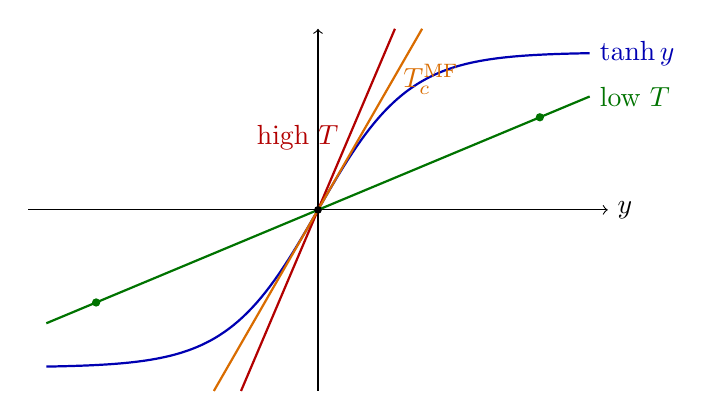
\begin{tikzpicture}[x=1.15cm,y=2.0cm]
\draw[->] (-3.2,0) -- (3.2,0) node[right] {$y$};
\draw[->] (0,-1.15) -- (0,1.15);
\draw[thick,blue!70!black,domain=-3:3,samples=120]
  plot (\x,{tanh(\x)}) node[right] {$\tanh y$};
\draw[thick,red!70!black] (-0.85,-1.15) -- (0.85,1.15)
  node[pos=0.70,left] {high \(T\)};
\draw[thick,orange!85!black] (-1.15,-1.15) -- (1.15,1.15)
  node[pos=0.86,right] {\(T_c^{\rm MF}\)};
\draw[thick,green!45!black] (-3,-0.72) -- (3,0.72)
  node[right] {low \(T\)};
\fill (0,0) circle (1.4pt);
\fill[green!45!black] (-2.45,-0.588) circle (1.5pt);
\fill[green!45!black] (2.45,0.588) circle (1.5pt);
\end{tikzpicture}
\caption{Eine normierte Rekonstruktion der grafischen Selbstkonsistenzargumentation.}
\end{figure}

Der von null verschiedene Lösungszweig entsteht kontinuierlich. In der Nähe des Übergangs gilt
\begin{equation}
\tanh(Km)=Km-\frac{(Km)^3}{3}+O(m^5).
\end{equation}
Für \(K>1\) erfüllen die kleinen, von null verschiedenen Lösungen
\begin{equation}
m^2\simeq \frac{3(K-1)}{K^3}.
\end{equation}
Das mittlere Feld sagt somit den bekannten wurzelförmigen Anstieg \(m\propto(T_c-T)^{1/2}\) voraus.

Die Stabilitätsaussage lässt sich auch formulieren, ohne sich auf die grafische Darstellung zu stützen. Bis auf eine von \(m\) unabhängige Konstante lautet die freie Energie pro Spin im mittleren Feld
\begin{equation}
f_{\rm MF}(m)
=dJm^2-\frac{1}{\beta}
\log\!\left[2\cosh(2\beta dJm)\right].
\label{eq:mf-free-energy}
\end{equation}
Ihre Stationaritätsbedingung ist
\begin{equation}
\frac{\partial f_{\rm MF}}{\partial m}
=2dJ\left[m-\tanh(2\beta dJm)\right]=0.
\end{equation}
Oberhalb von \(T_c^{\rm MF}\) ist \(m=0\) das Minimum. Unterhalb davon ist der Ursprung ein lokales Maximum, und die beiden von null verschiedenen Lösungen sind entartete Minima. Die Schnittpunktgeometrie und die Thermodynamik der freien Energie führen zur selben Aussage.

\begin{classroomqa}
\audiencequestion{Die Lösung \(m=0\) bleibt auch unterhalb von \(T_c^{\rm MF}\) ein Schnittpunkt. Warum sollte der von null verschiedene Zweig physikalisch sein?}
\lecturerresponse{Folgt man dem System von Temperatur null an nach oben, befindet es sich bereits auf einem magnetisierten Zweig. Genauer: Unterhalb des Übergangs hat die freie Energie im mittleren Feld Minima bei \(\pm m_0\), während \(m=0\) zu einem Maximum wird. Ein infinitesimales äußeres Feld wählt dann eines der Minima aus und hebt die scheinbare Mehrdeutigkeit auf. \lecturetimestamp{01:11:34--01:12:18}}
\end{classroomqa}

\section{Warum das mittlere Feld in einer Dimension versagt}

Setzt man \(d=1\) in Gleichung~\eqref{eq:mean-field-tc} ein, sagt das Modell einen Übergang bei \(T=2J\) voraus, im Widerspruch zur exakten eindimensionalen Lösung. Algebraisch wird dabei nichts singulär. Die Näherung versagt, weil zwei Nachbarn kein großes statistisches Reservoir bilden und Domänenwände in einer Dimension eine ungewöhnlich große Entropie besitzen.

Wir beginnen im Zustand, in dem alle Spins nach oben zeigen. Eine aufgebrochene Bindung ändert ihre Energie von \(-J\) zu \(+J\), sodass jede aufgebrochene Bindung Energie kostet:
\begin{equation}
\Delta E_{\rm bond}=2J.
\end{equation}
Auf einem quadratischen Gitter unterbricht das Umklappen eines einzelnen Spins vier Bindungen und kostet \(8J\). Bei zwei benachbarten umgeklappten Spins umfasst der Rand sechs aufgebrochene Bindungen und kostet \(12J\), während zwei weit voneinander entfernte Umklappungen acht Bindungen unterbrechen und \(16J\) kosten.

\begin{figure}[ht]
\centering
\includegraphics[width=0.82\textwidth]{lecture_09_figure_09.png}
\caption{Zwei benachbarte umgekehrte Spins auf einem quadratischen Gitter; ihre gemeinsame Bindung ist erfüllt, sodass ein Rand aus sechs Bindungen bleibt.}
\lectureframe{01:17:30}
\end{figure}

Ein kompakter umgekehrter Bereich kostet in zwei Dimensionen daher eine Energie proportional zu seiner Randlänge:
\begin{equation}
\Delta E_{\rm 2d}=2J\,|\partial D|.
\end{equation}
Wächst der Bereich, wächst im Allgemeinen auch sein Rand.

In einer Dimension ist es anders. Ein zusammenhängender umgekehrter Block hat unabhängig von seiner Länge nur zwei Domänenwände:
\begin{equation}
\Delta E_{\rm 1d}=2(2J)=4J.
\label{eq:one-d-domain-cost}
\end{equation}

\begin{figure}[ht]
\centering
\includegraphics[width=0.82\textwidth]{lecture_09_figure_10.png}
\caption{Ein langer umgekehrter Block in einer Dimension, begrenzt von nur zwei Domänenwänden.}
\lectureframe{01:19:10}
\end{figure}

In einer Kette mit \(N\) Gitterplätzen gibt es von der Größenordnung \(N^2\) Möglichkeiten, die beiden Wände eines solchen Blocks zu wählen. Seine Energie wächst nicht mit dem Abstand zwischen den Wänden. Bei jeder positiven Temperatur ermöglicht die Entropie daher beliebig große umgekehrte Domänen. In zwei Dimensionen kann die Energie des Randes die Konturentropie bei hinreichend niedriger Temperatur überwinden. Dieser Wettbewerb zwischen Energie und Entropie ist der geometrische Umstand, den das mittlere Feld nicht erfasst, wenn es \(d=1\) und \(d=2\) lediglich als verschiedene Zahlenwerte desselben Koeffizienten behandelt.

\begin{classroomqa}
\audiencequestion{Setzt der konstante Energieaufwand für zwei Domänenwände voraus, dass die umgeklappten Spins benachbart sind?}
\lecturerresponse{Ja. Die Aussage bezieht sich auf einen einzelnen zusammenhängenden umgekehrten Block. Bilden die umgeklappten Spins mehrere getrennte Blöcke, entstehen für jeden Block zwei zusätzliche Domänenwände. Entscheidend ist, dass ein einzelner Block beliebig lang sein kann und dennoch nur zwei Wände besitzt. \lecturetimestamp{01:18:32--01:18:40}}
\end{classroomqa}

\begin{classroomqa}
\audiencequestion{Die Gleichung im mittleren Feld scheint selbst keinen qualitativen Unterschied zwischen \(d=1\) und \(d=2\) zu zeigen. Ist das das Problem?}
\lecturerresponse{Genau. Das mittlere Feld sagt für jedes positive \(d\) einen Übergang voraus und ist daher in einer Dimension qualitativ falsch. Bei der Herleitung wurden viele schwach fluktuierende Nachbarn vorausgesetzt und die Geometrie der Domänenwände vernachlässigt. Für den eindimensionalen Fall entscheidet die exakte Bindungslösung, nicht die Ersetzung im mittleren Feld \(d=1\). \lecturetimestamp{01:19:44--01:20:28}}
\end{classroomqa}

\section{Ein äußeres Feld wählt die Phase aus}

Wir ergänzen ein homogenes Feld \(h\) mit der Konvention, dass \(h>0\) den Zustand \(\sigma=+1\) begünstigt:
\begin{equation}
H=-J\sum_{\langle ij\rangle}\sigma_i\sigma_j
-h\sum_i\sigma_i.
\label{eq:ising-with-field}
\end{equation}
Die Energie des ausgewählten Spins im mittleren Feld lautet
\begin{equation}
E_i^{\rm MF}=-(2dJm+h)\sigma_i,
\end{equation}
und die Selbstkonsistenzgleichung wird zu
\begin{equation}
\boxed{m=\tanh\!\left[\beta(2dJm+h)\right]}.
\label{eq:self-consistency-field}
\end{equation}
Mit \(K=2\beta dJ\) und \(y=Km\) gilt
\begin{equation}
\frac{y}{K}=\tanh(y+\beta h).
\label{eq:shifted-graph}
\end{equation}

\begin{figure}[ht]
\centering
\includegraphics[width=0.82\textwidth]{lecture_09_figure_11.png}
\caption{Der zur Selbstkonsistenzgleichung hinzugefügte Term des äußeren Feldes und die entsprechend verschobene grafische Konstruktion.}
\lectureframe{01:26:20}
\end{figure}

\begin{classroomqa}
\audiencequestion{Warum wird das Feld nur innerhalb des hyperbolischen Tangens hinzugefügt? Müsste es nicht auch die linke Seite verändern?}
\lecturerresponse{Die linke Seite ist die angenommene Magnetisierung \(m\), gleichbedeutend mit \(y/K\). Die rechte Seite ist die für einen Spin im gesamten effektiven Feld \(2dJm+h\) berechnete Magnetisierung. Die Selbstkonsistenz setzt diese beiden Größen gleich. Hält man \(y=Km\) als Definition fest, erscheint der neue Term nur im Argument \(\tanh(y+\beta h)\). \lecturetimestamp{01:23:46--01:26:18}}
\end{classroomqa}

\begin{classroomqa}
\audiencequestion{Lässt sich dieselbe grafische Änderung auch dadurch beschreiben, dass man die Geraden verschiebt, statt die Kurve \(\tanh\) zu verschieben?}
\lecturerresponse{Ja. Man kann \(\tanh y\) festhalten und die Gleichung so umschreiben, dass die Gerade einen von null verschiedenen Achsenabschnitt hat. Die Schnittpunkte sind dieselben. Die beiden Beschreibungen unterscheiden sich nur darin, welche Seite der Gleichung als feste Kurve gewählt wird. \lecturetimestamp{01:35:07--01:36:26}}
\end{classroomqa}

Für \(h\neq0\) ist der Ursprung keine Lösung mehr. Unterhalb von \(T_c^{\rm MF}\) wählt ein beliebig kleines positives Feld den positiven Zweig, ein negatives Feld den negativen.

\begin{figure}[ht]
\centering
\includegraphics[width=0.82\textwidth]{lecture_09_figure_12.png}
\caption{Ein schwaches Feld hebt den symmetrischen Schnittpunkt auf und wählt einen der magnetisierten Zweige aus.}
\lectureframe{01:36:22}
\end{figure}

Die korrekte Aussage setzt eine Reihenfolge der Grenzübergänge voraus. Bei einem endlichen System mit genau \(h=0\) besitzt das Gleichgewicht Spin-Umkehrsymmetrie, daher gilt im vollständigen Gleichgewichtsensemble \(\expect{m}=0\). Die spontane Magnetisierung ist definiert als
\begin{equation}
m_{\rm sp}
=\lim_{h\to0^+}\lim_{N\to\infty}\expect{m}_{N,h},
\end{equation}
wobei zuerst der thermodynamische Grenzfall genommen wird. Eine Umkehr des Vorzeichens des infinitesimalen Feldes ergibt \(-m_{\rm sp}\). Die Differenz der gesamten Feldenergie ist proportional zu \(Nh\), sodass selbst ein winziges Feld für eine makroskopische Probe ausschlaggebend wird.

An der zugehörigen freien Energie wird die Neigung sichtbar:
\begin{equation}
f_{\rm MF}(m;h)
=dJm^2-\frac{1}{\beta}
\log\!\left[2\cosh\!\left(\beta(2dJm+h)\right)\right].
\end{equation}
Bei \(h=0\) sind die beiden Minima gleich tief. Ein positives \(h\) senkt das Minimum bei positivem \(m\) und hebt das bei negativem \(m\) an. Die Störung pro Spin kann winzig sein, während die mit \(N\) multiplizierte Gesamtbevorzugung makroskopisch ist.

\begin{classroomqa}
\audiencequestion{Wenn das äußere Feld bestehen bleibt, ist die Magnetisierung dann wirklich spontan?}
\lecturerresponse{Das Feld dient nur dazu, einen der beiden Zweige auszuwählen. Bei festem \(T<T_c\) lässt man das System unendlich groß werden und anschließend \(h\to0^+\). Die Magnetisierung bleibt endlich, obwohl das Auswahlfeld verschwindet. Mit umgekehrtem Vorzeichen des Grenzübergangs wird die entgegengesetzte Phase ausgewählt. \lecturetimestamp{01:33:15--01:34:18}}
\end{classroomqa}

\begin{classroomqa}
\audiencequestion{Ist die Lösung mit verschwindendem Mittelwert unterhalb des Übergangs tatsächlich unmöglich oder lediglich instabil?}
\lecturerresponse{Bei exakt verschwindendem Feld ist ein symmetrisches Ensemble endlichen Volumens mit gleichem Gewicht für beide Orientierungen möglich; sein Mittelwert ist null. Was nicht stabil ist, ist eine solche Konfiguration als einzelne makroskopische Phase. Ein beliebig kleines Feld verändert die extensive Energiebilanz und wählt eine Orientierung aus; nach dem thermodynamischen Grenzübergang bleibt die ausgewählte Magnetisierung bestehen, wenn das Feld wieder entfernt wird. \lecturetimestamp{01:34:25--01:35:06}}
\end{classroomqa}

\begin{classroomqa}
\audiencequestion{Was geschieht bei unendlicher Temperatur mit der durch das Feld verzerrten Lösung?}
\lecturerresponse{Für jedes feste endliche \(h\) verschwinden sowohl \(K=2\beta dJ\) als auch \(\beta h\) für \(T\to\infty\). Gleichung~\eqref{eq:self-consistency-field} liefert dann \(m\to0\). Das schwache Feld wählt einen Tieftemperaturzweig aus, kann die Ordnung aber nicht gegen unendliche thermische Fluktuationen aufrechterhalten. \lecturetimestamp{01:27:39--01:29:51}}
\end{classroomqa}

\begin{classroomqa}
\audiencequestion{Wenn Temperatur und die Verschiebung der Kurve gleichzeitig verändert werden, wie lässt sich sicher feststellen, wohin sich der Schnittpunkt bewegt?}
\lecturerresponse{Die implizite Gleichung ist verlässlicher als die sich verschiebende Skizze. Bei niedriger Temperatur und positivem \(h\) nähert sich ihre stabile Lösung \(m=+1\). Bei hoher Temperatur ergibt die Entwicklung des Tangens
\[
m\simeq \beta(2dJm+h)
\quad\Longrightarrow\quad
m\simeq \frac{\beta h}{1-2\beta dJ},
\]
Dieser Ausdruck geht gegen null, wenn \(\beta\to0\). Der stabile Zweig verbindet somit den ausgerichteten Tieftemperaturgrenzfall mit dem schwach polarisierten Hochtemperaturgrenzfall, ohne unterhalb des Übergangs im instabilen Ursprung zu verharren. \lecturetimestamp{01:29:53--01:33:04}}
\end{classroomqa}

\section{Eine magnetische Umkehr ist ein anderes Problem}

\begin{classroomqa}
\audiencequestion{Was bewirkt eine Umkehr der Richtung des Erdmagnetfelds?}
\lecturerresponse{Diese Frage liegt außerhalb des Gleichgewichts-Ising-Modells. Das Hauptfeld der Erde wird durch den Geodynamo erzeugt: Konvektion und Rotation elektrisch leitfähiger Flüssigkeit im äußeren Kern erhalten elektrische Ströme und ein Magnetfeld aufrecht. Umkehrungen sind unregelmäßige Neuordnungen dieses nichtlinearen Dynamos und keine einfache Umkehr einer ferromagnetischen Domäne in festem Eisen. Ihr genauer zeitlicher Verlauf lässt sich nicht durch einen einzigen Gleichgewichts-Ordnungsparameter erfassen. Die ehrliche Antwort lautet daher: Die Ising-Rechnung erklärt den Auslöser nicht. Der nützliche Zusammenhang ist lediglich allgemeiner Art: Ein System mit zwei entgegengesetzten großräumigen Orientierungen kann zwischen ihnen instabil werden.\footnote{Siehe den \href{https://science.nasa.gov/science-research/earth-science/earths-magnetosphere-protecting-our-planet-from-harmful-space-energy/}{NASA-Überblick zum Geodynamo} und die \href{https://www.usgs.gov/programs/geomagnetism/introduction-geomagnetism}{Einführung des USGS in den Geomagnetismus}.} \lecturetimestamp{01:38:39--01:40:32}}
\end{classroomqa}

Die exakte Kette und das Gitter in der Mittelwertnäherung liefern nun zwei deutlich unterschiedliche Antworten. In einer Dimension gilt
\begin{equation}
\expect{\sigma_i\sigma_{i+r}}
=\left[\tanh(\beta J)\right]^r
\longrightarrow0
\qquad (T>0),
\end{equation}
da Domänenwände mit endlicher Energie beliebig lange umgekehrte Bereiche voneinander trennen können. Bei vielen Nachbarn lässt das selbstkonsistente Feld dagegen unterhalb von
\begin{equation}
T_c^{\rm MF}=2dJ.
\end{equation}
stabile, von null verschiedene Lösungen zu. Der Unterschied ist nicht bloß algebraischer Art. Entscheidend ist das Zusammenspiel von Geometrie, Energie, Entropie und Redundanz: ob sich ein Fehler ungehindert ausbreiten kann oder ob das umgebende Gitter ihn korrigieren kann.